% Préambule APMEP - Annales
% Auteurs
% tapuscrit : 			
% relecture :
% figures TikZ :
% figures pstricks :
% modifications :
% Remerciements :
% version 1 : 2026-09-14
%
\documentclass[12pt,a4paper,french]{article}

% Packages
%%% codage et police utilisée
\usepackage[T1]{fontenc}
\RequirePackage{iftex}
\iftutex % moteur utf-8 lualatex, xelatex
	\usepackage{fourier-otf} % remplace fourier pour moteur utf8 (LuaLaTeX, XeLaTeX)
	% Alternatives nécéssite (LuaLaTeX, XeLaTeX)
    \usepackage{hyperref}
	%\usepackage{fontspec}% pour utiliser des fontes système
\else % pour les autres moteurs latex, pdflatex
	\usepackage[utf8]{inputenc}
	\usepackage{fourier}
	\usepackage{amsmath,amssymb}
    \usepackage[dvips]{hyperref}
    \renewcommand{\ttdefault}{lmtt}
\fi
\usepackage[normalem]{ulem}
\usepackage{pifont}
\usepackage{lscape}
% tableaux
\usepackage{multicol}
\usepackage{multirow}
\usepackage{tabularx}
\usepackage{tabularray}
% texte et composition
\usepackage{textcomp}
\usepackage{babel}
\usepackage[np]{numprint}
%
\usepackage{fancyhdr}
\usepackage{makeidx}
\makeindex
% pour le symbole €
\usepackage{eurosym}
\DeclareRobustCommand{\officialeuro}{%
  \ifmmode\expandafter\text\fi
  {\fontencoding{U}\fontfamily{eurosym}\selectfont e}}
\AtBeginDocument{\renewcommand{\euro}{\officialeuro}}
% couleurs étendues
\usepackage{xcolor}
% pour les listes
\usepackage{enumitem}
% Enumérations réglage par défaut
\setlist[itemize]{label=\textbullet,leftmargin=5mm,labelwidth=3mm,labelsep=2mm,align=left}
\setlist[enumerate]{labelindent=0pt, leftmargin=5mm, labelsep=2mm, labelwidth=3mm,labelsep=2mm, align= left}
\setlist[enumerate,1]{label = \textbf{\arabic*.}}
\setlist[enumerate,2]{label = \textbf{\alph*.}}
\setlist[enumerate,3]{label = \textbf{\roman*.}}
% pour l'ajustement des boites (figures…)
\usepackage{adjustbox}
% pour ne pas commencer un exercice en fin de page
\usepackage{needspace}
%
% Taille de la zone d'écriture
\usepackage[left=1.5cm,right=1.5cm,top=2.5cm,bottom=2.5cm]{geometry}
\setlength{\headheight}{15pt}
\setlength{\parindent}{0mm}
%
% Formatage du pdf
\hypersetup{%
    pdfauthor = {APMEP},
    pdfsubject = {Troisième, Série générale},
    pdftitle = {Brevet des collèges -- Polynésie Remplacement -- 7 septembre 2026},
    allbordercolors = white,
    pdfstartview=FitH
}
\usepackage{graphicx}
% Pour scratch (code)
\usepackage{scratch3}
% Pour le code Python
\usepackage{listings}
\lstdefinestyle{python}{
  language=Python,
  basicstyle=\ttfamily\small,
  keywordstyle=\color{blue}\bfseries,
  commentstyle=\color{gray}\itshape,
  stringstyle=\color{orange},
  numbers=left,
  numberstyle=\tiny\color{gray},
  breaklines=true,
  frame=single,
  backgroundcolor=\color{gray!5},
  tabsize=4
}
% Pour une visualisation de type tableur
\usepackage{pas-tableur}
%
%% pour PsTricks
\usepackage{pst-bezier}%% AVANT les autres PST
\usepackage{pstricks-add}
\usepackage{pst-func,pst-tree,pst-circ}
\usepackage{pst-eucl}
%% pour TikZ
\usepackage{tikz,pgfplots,pgf,tkz-tab,tikzpagenodes}
\usetikzlibrary{calc,patterns,decorations.markings,arrows.meta,patterns.meta,arrows}
\tikzset{
    singletick/.style={
        postaction={decorate,decoration={markings,mark=at position 0.5 with {
            \draw[line width=1pt] (0,-3pt) -- (0,3pt);
        }}}
    },
    doubletick/.style={
        postaction={decorate,decoration={markings,mark=at position 0.5 with {
            \draw[line width=1pt] (-1pt,-3pt) -- (-1pt,3pt);
            \draw[line width=1pt] (1pt,-3pt) -- (1pt,3pt);
        }}}
    }
}
\pgfplotsset{compat=1.18,/pgf/number format/.cd,use comma}
\usepackage{icomma} % gestion des espaces autour des virgules
\DeclareMathSymbol{;}{\mathbin}{operators}{"3B}% pour un espacement correct du ; en mode maths
%%%%%%%%%%%%%%%%%%%%%%%%%%%%%%%%%%%%%%%%%%
% Définitions
%
% notation en mode mathématique et hors mode mathématique
\newcommand{\R}{\ensuremath{\mathbb{R}}}
\newcommand{\N}{\ensuremath{\mathbb{N}}}
\newcommand{\D}{\ensuremath{\mathbb{D}}}
\newcommand{\Z}{\ensuremath{\mathbb{Z}}}
\newcommand{\Q}{\ensuremath{\mathbb{Q}}}
\newcommand{\C}{\ensuremath{\mathbb{C}}}
%
\providecommand{\up}{\textsuperscript}
%
\newcommand{\vect}[1]{\overrightarrow{\,\mathstrut#1\,}}
\newcommand{\vectt}[1]{\overrightarrow{\,\mathstrut\text{#1}\,}}
%
\def\Oij{$\left(\text{O};\vect{\imath},\vect{\jmath}\right)$}
\def\Oijk{$\left(\text{O};\vect{\imath},\vect{\jmath},\vect{k}\right)$}
\def\Ouv{$\left(\text{O};\vect{u},\vect{v}\right)$}
%
\newcommand{\ds}{\displaystyle}
%
\renewcommand{\d}{\mathrm{\,d}}
\renewcommand{\i}{\mathrm{\,i\,}}
\newcommand{\e}{\mathrm{\,e\,}}
%%%%%%%%%%%%%%%%%%%%%%%%%%%%%%%%%%%%%%%%%%%


\begin{document}

%---------------------------------------------------------
% Réglage entête, pied de page
%---------------------------------------------------------
\rhead{\textbf{A. P{}. M. E. P{}.}}
\lhead{\small Sujet}
\lfoot{\small{Polynésie -- Remplacement}}
\rfoot{\small{7 septembre 2026}}
\pagestyle{fancy}

\thispagestyle{empty}


%---------------------------------------------------------
% Titre
%---------------------------------------------------------
\begin{center}
{\Large \textbf{
		\decofourleft~ Diplôme National du Brevet ~\decofourright\\[10pt]
		Série générale -- Polynésie (Remplacement) -- 7 septembre 2026
		\marginpar{\rotatebox{90}{\textbf{A. P{}. M. E. P{}.}}}\\[10pt]
		Sujet\\[10pt]}}
\end{center}

\begin{center}
\textbf{Durée : 2 heures} \qquad \textbf{Coefficient : 2}
\end{center}

L'usage de la calculatrice avec mode examen actif ou sans mémoire \og type collège \fg{} est \textbf{interdit} pour la partie 1 et \textbf{autorisé} pour la partie 2.

L'utilisation du dictionnaire est interdite.

\bigskip

\section*{\centering PREMIÈRE PARTIE : AUTOMATISMES (6 pts)}

Pour chaque question, recopier sur la copie son numéro et la réponse correspondante.

Pour cette partie, aucune justification n'est demandée.

Pour les questions à choix multiple, une seule réponse est exacte.

\subsection*{Question 1}
Réduire l'expression $A = 4x + 3x$.

\subsection*{Question 2}
Déterminer la médiane de la série statistique suivante : $8$ ; $18$ ; $17$ ; $3$ ; $7$.

\subsection*{Question 3}
Calculer $25\,\%$ de $160$~\euro.

\subsection*{Question 4}
Un triangle est formé d'un angle de $60^{\circ}$ et d'un autre de $100^{\circ}$. Déterminer la mesure, en degré, du troisième angle.

\subsection*{Question 5}
\begin{minipage}{0.63\linewidth}
Recopier sur la copie et compléter par des longueurs des côtés du triangle DEF pour que l'égalité ci-dessous soit vraie :
\[\cos\left(\widehat{\mathrm{DEF}}\right) = \dfrac{\dots}{\dots}\]
\end{minipage}\hfill
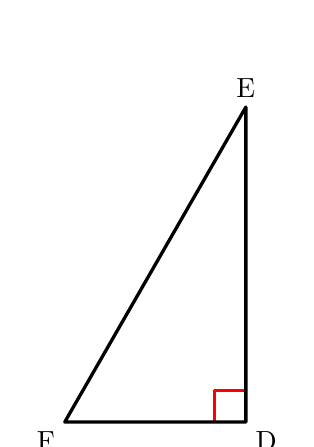
\begin{tikzpicture}[rotate=0,line cap=round, line join=round,baseline={(current bounding box.center)}]
\coordinate (D) at (0,0);
\coordinate (E) at (0,4);
\coordinate (F) at (-2.3,0);
\draw[line width=1pt,red] (0,0) rectangle (-0.4,0.4) ;
\draw[line width=1.2pt] (D) -- (E) -- (F) -- cycle;
\node[below right] at (D) {D};
\node[above] at (E) {E};
\node[below left] at (F) {F};
\end{tikzpicture}

\subsection*{Question 6}
Développer et réduire l'expression $a(3a - 2)$.

\subsection*{Question 7}
Quatre élèves proposent une justification pour montrer que \np{4836} est divisible par 3. Recopier sur la copie le numéro de l'élève qui a justifié correctement.

\begin{center}
\begin{tblr}{*{4}{|X[c]}|}
	\hline
	\textbf{Élève 1} & \textbf{Élève 2} & \textbf{Élève 3} & \textbf{Élève 4} \\
	Le chiffre des unités de \np{4836} est 6, qui est un multiple de 3. & La somme des chiffres de \np{4836} est divisible par 3. & \np{4836} est un nombre pair. & 36 est divisible par 3. \\
	\hline
\end{tblr}
\end{center}

\subsection*{Question 8}
Recopier sur la copie le calcul donnant l'aire, en cm$^2$, d'un disque de diamètre 6 cm.

\begin{center}
\begin{tblr}{*{4}{|X[c]}|}
	\hline
	$\pi \times 6^2$ & $\pi \times 3^2$ & $2 \times \pi \times 3$ & $2 \times \pi \times 6$ \\
	\hline
\end{tblr}
\end{center}

\subsection*{Question 9}
Recopier sur la copie l'expression en fonction de $x$ qui correspond au périmètre du polygone ACDEFB.

\begin{center}
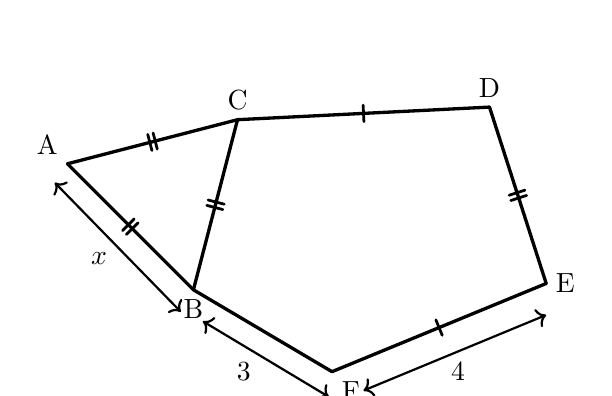
\begin{tikzpicture}[line cap=round, line join=round, scale=0.8]
	\coordinate (A) at (0,3);
	\coordinate (B) at (2,1);
	\coordinate (C) at (2.7,3.7);
	\coordinate (D) at (6.7,3.9);
	\coordinate (E) at (7.6,1.1);
	\coordinate (F) at (4.2,-0.3);
	
	% Tracé des segments avec les codages respectifs
	\draw[line width=1.2pt, doubletick] (A) -- (B);
	\draw[line width=1.2pt] (B) -- (F);
	\draw[line width=1.2pt, singletick] (F) -- (E);
	\draw[line width=1.2pt, doubletick] (E) -- (D);
	\draw[line width=1.2pt, singletick] (D) -- (C);
	\draw[line width=1.2pt, doubletick] (C) -- (A);
	\draw[line width=1.2pt, doubletick] (B) -- (C);
	
	% Doubles flèches pour les dimensions (entre la figure et les textes)
	\draw[<->, line width=0.8pt] (-0.2, 2.7) -- (1.8, 0.65);
	\draw[<->, line width=0.8pt] (2.15, 0.5) -- (4.15, -0.7);
	\draw[<->, line width=0.8pt] (4.7, -0.6) -- (7.6, 0.6);
	
	\node[above left] at (A) {A};
	\node[below] at (B) {B};
	\node[above] at (C) {C};
	\node[above] at (D) {D};
	\node[right] at (E) {E};
	\node[below right] at (F) {F};
	\node at (0.5,1.5) {$x$};
	\node at (2.8,-0.3) {3};
	\node at (6.2,-0.30) {4};
\end{tikzpicture}
\end{center}

\begin{center}
\begin{tblr}{*{4}{|X[c]}|}
	\hline
	$4x + 11$ & $x^3 + 11$ & $x + 7$ & $3x + 11$ \\
	\hline
\end{tblr}
\end{center}

\begin{center}
\emph{Restitution de la copie du candidat à l'issue de la partie 1}
\end{center}

\newpage
\section*{\centering DEUXIÈME PARTIE : RAISONNEMENT ET RÉSOLUTION DE PROBLÈMES (14 pts)}

\begin{quote}
\emph{Dans cette partie, toutes les réponses doivent être justifiées, sauf si une indication contraire est donnée.\\
	La clarté et la précision des raisonnements ainsi que la rédaction sont évaluées sur 2 points.\\
	Pour chaque question, si le travail n'est pas terminé, laisser tout de même une trace de la recherche ; les essais et les démarches engagées, même non aboutis, seront pris en compte dans la notation.}
\end{quote}

\needspace{10\baselineskip}
\section*{Exercice 1 \hfill 3,5 points}

On dispose d'une boîte opaque contenant 7 boules blanches identiques et indiscernables au toucher. Les boules sont numérotées de 1 à 7.

\begin{enumerate}
	\item On s'intéresse aux boules dont le numéro est un nombre premier.
	\begin{enumerate}
		\item Citer les numéros de boules correspondant à des nombres premiers.
		\item Vérifier que la probabilité d'obtenir une boule dont le numéro est un nombre premier est de $\dfrac{4}{7}$.
	\end{enumerate}
	\item On réalise l'expérience suivante : \og On tire au sort une boule de la boîte, on note le numéro qu'elle porte puis on remet la boule dans la boîte \fg.
	
	On répète cette expérience 100 fois. Le diagramme en bâtons ci-après représente la fréquence d'apparition de chacun des numéros.

\begin{center}
		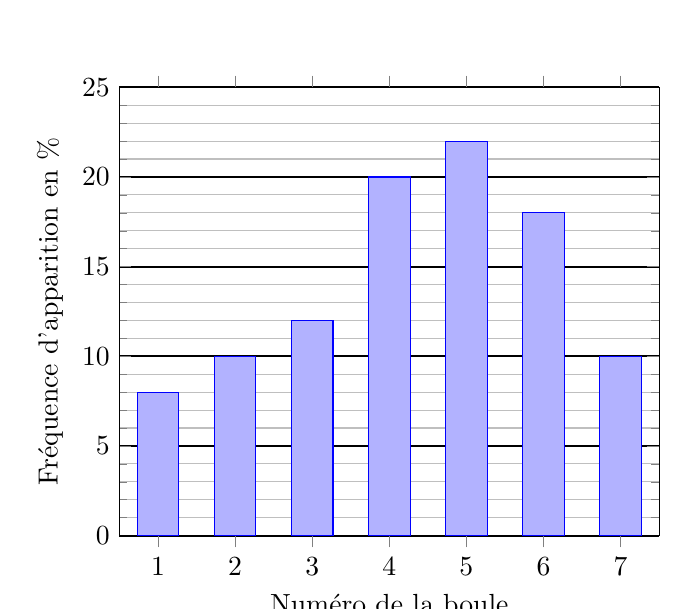
\begin{tikzpicture}
			\begin{axis}[
				title={},
				xlabel={Numéro de la boule},
				ylabel={Fréquence d'apparition en \%},
				xmin=0.5, xmax=7.5,
				ymin=0, ymax=25,
				ytick={0,5,10,15,20,25},
				ymajorgrids=true,                  
				major grid style={black, thick},   
				yminorgrids=true,                  
				minor y tick num=4,                
				minor grid style={lightgray},      
				ybar,
				bar width=15pt
			]
			\addplot coordinates {(1,8) (2,10) (3,12) (4,20) (5,22) (6,18) (7,10)};
			\end{axis}
		\end{tikzpicture}
	\end{center}

	\begin{enumerate}
		\item En utilisant ce diagramme en bâtons, déterminer la fréquence d'apparition de la boule qui porte le numéro 2.
		\item Vérifier que la somme des fréquences d'apparition des boules dont le numéro est un nombre premier est égale à $54\,\%$.
	\end{enumerate}
	\item D'après les questions précédentes, on dispose des informations suivantes :
	\begin{itemize}
		\item la probabilité d'obtenir un nombre premier est $\dfrac{4}{7}$ ;
		\item la fréquence d'apparition d'un nombre premier est de $54\,\%$.
	\end{itemize}
	\begin{enumerate}
		\item Montrer que $\dfrac{4}{7}$ n'est pas égal à $54\,\%$.
		\item Expliquer pour quelle raison la probabilité calculée et la fréquence d'apparition mesurée ne donnent pas la même valeur.
	\end{enumerate}
\end{enumerate}

\needspace{10\baselineskip}
\section*{Exercice 2 \hfill 4 points}

On considère la figure géométrique ci-dessous qui n'est pas en vraie grandeur.

Les points G, A, O, C et E sont alignés.

Les points B, O, D et F sont alignés.

COD est un triangle rectangle en O.

$\mathrm{OD} = 4$ cm, $\mathrm{OB} = 6$ cm, $\mathrm{OC} = 3$ cm, $\mathrm{CE} = 1{,}5$ cm et $\mathrm{DF} = 2$ cm.

La droite (BF) est l'axe de symétrie de cette figure.

\begin{center}
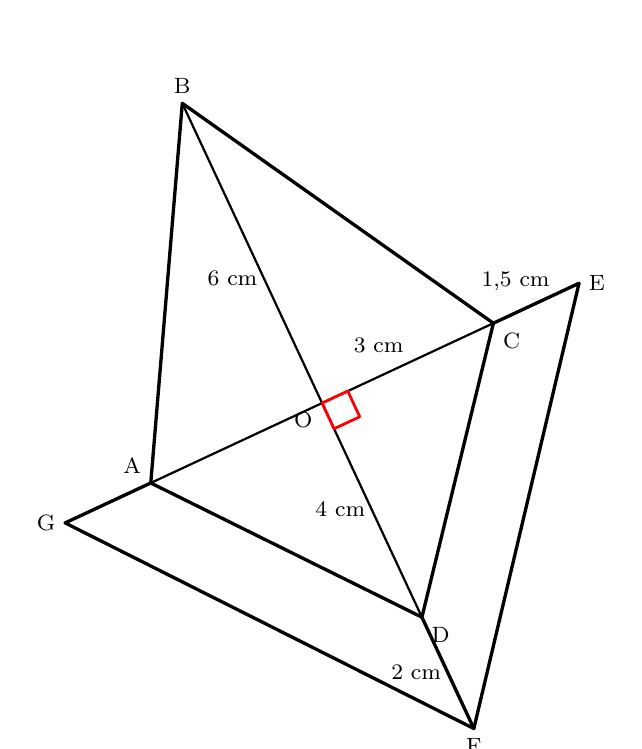
\begin{tikzpicture}[rotate=25,scale=1.2, line cap=round, line join=round, font=\footnotesize]
	\coordinate (O) at (0,0);
	\coordinate (C) at (2,0);
	\coordinate (A) at (-2,0);
	\coordinate (D) at (0,-2.5);
	\coordinate (B) at (0,3.5);
	\coordinate (E) at (3,0);
	\coordinate (F) at (0,-3.8);
	\coordinate (G) at (-3,0);
	\draw[line width=1.2pt] (A) -- (B) -- (C) -- (D) -- cycle;
	\draw[line width=1.2pt] (A) -- (G) -- (F) -- (D);
	\draw[line width=1.2pt] (C) -- (E) -- (F);
	\draw[line width=0.8pt] (G) -- (E);
	\draw[line width=0.8pt] (B) -- (F);
	\node[above left] at (A) {A};
	\node[above] at (B) {B};
	\node[below right] at (C) {C};
	\node[below right] at (D) {D};
	\node[right] at (E) {E};
	\node[below] at (F) {F};
	\node[left] at (G) {G};
	\node[below left] at (O) {O};
	\draw[red, line width=1pt] (0,0) rectangle (0.3,-0.3);
	
	\node at (0.8,0.3) {$3$ cm};
	\node at (2.4,0.3) {$1,5$ cm};
	\node at (-0.3,1.6) {$6$ cm};
	\node at (-0.3,-1.1) {$4$ cm};
	\node at (-0.3,-3) {$2$ cm};
\end{tikzpicture}
\end{center}

\begin{enumerate}
	\item Justifier que $\mathrm{OA} = 3$ cm.
	\item Sur la copie, construire en vraie grandeur le quadrilatère ABCD.
	\item En se plaçant dans le triangle OFE, calculer la longueur du côté [FE].
	\item Démontrer que les droites (CD) et (EF) sont parallèles.
\end{enumerate}

\needspace{10\baselineskip}
\section*{Exercice 3 \hfill 3 points}

Voici un tableau des températures moyennes annuelles à Paris, mesurées par une station météorologique entre 2015 et 2024. Les températures sont exprimées en degré Celsius ($^{\circ}$C).

\begin{center}
\begin{tblr}{hline{1,3}=1pt,vlines,colspec={|c|c|c|c|c|c|c|c|c|c|c|}}
	\hline
Année & 2015 & 2016 & 2017 & 2018 & 2019 & 2020 & 2021 & 2022 & 2023 & 2024 \\
	\hline
Température ($^{\circ}$C) & 13,47 & 12,87 & 13,39 & 13,91 & 13,66 & 14,28 & 12,86 & 14,30 & 14,27 & 13,50 \\
	\hline
\end{tblr}
\end{center}
\small{Source : \url{https://opendata.paris.fr/explore/dataset/temperature_moyenne_paris/table/?sort=annee}}
%\normalsize

\begin{enumerate}
\item
	\begin{enumerate}
		\item Calculer l'étendue de la série des températures moyennes annuelles de 2015 à 2024.
		\item Recopier sur la copie la formule qui doit être saisie dans la cellule L2 pour obtenir la température minimale de 2015 à 2024.
		
\begin{center}
\begin{tblr}{*{4}{|X[c]}|}
			\hline
			\texttt{=MIN(B1:K1)} & \texttt{=MIN(B2:K2)} & \texttt{=MIN(B2:L2)} & \texttt{=MIN(B1:L1)} \\
			\hline
\end{tblr}
\end{center}
	\end{enumerate}
\item La température moyenne annuelle à Paris en 1924 était de $10{,}73^{\circ}$C tandis que celle de 2024 était de $13{,}50^{\circ}$C. Un élève affirme qu'en passant de 10,73 à 13,50, l'augmentation est supérieure à $25\,\%$. A-t-il raison ? Argumenter votre réponse en expliquant la démarche.
\end{enumerate}

Pour la suite du problème, on estime que la température moyenne annuelle à Paris augmente d'environ $0{,}025^{\circ}$C chaque année.

\begin{enumerate}
	\setcounter{enumi}{2}
	\item En 2024, la température moyenne à Paris était de $13{,}50^{\circ}$C. En se basant sur l'estimation annoncée ci-dessus, vérifier que la température moyenne à Paris en 2034 est estimée à $13{,}75^{\circ}$C.
	\item \textbf{(Question algorithmique)}\\
	L'objectif du programme ci-dessous, réalisé avec le logiciel Scratch, est d'estimer la température moyenne à Paris pour une année choisie.

	\begin{center}
	\begin{scratch}[scale=0.9,num blocks]
		\blockinit{Quand \greenflag est cliqué}
		\blocksensing{demander \ovalnum{Choisir un nombre supérieur à 2024} et attendre}
		\blockvariable{mettre \selectmenu{Nombre d'années d'écart} à \ovaloperator{\ovalvariable{réponse} - \ovalnum{2024}}}
		\blockvariable{mettre \selectmenu{Température} à \ovaloperator{\ovalnum{13.5} + \ovalnum{0.025} * \ovalvariable{Nombre d'années d'écart}}}
		\blocklook{dire \ovaloperator{regrouper\ovalnum{ La température en degré Celsius sera de} et {\ovalvariable{Température}}}}
	\end{scratch}
	\end{center}

	Un utilisateur choisit 2044 comme nombre de départ. Quelle valeur est alors stockée dans la variable \texttt{Nombre d'années d'écart} ?
	\item 
	\begin{enumerate}
		\item Résoudre l'équation : $13{,}5 + 0{,}025x = 15$.
		\item En quelle année la température moyenne annuelle à Paris sera-t-elle estimée à $15^{\circ}$C ?
	\end{enumerate}
\end{enumerate}

\needspace{10\baselineskip}
\section*{Exercice 4 \hfill 1,5 points}

Pour ses vacances, Riley se rend à Madrid en voiture et empruntera des autoroutes à péages.

\begin{enumerate}
	\item Le GPS lui indique un temps de trajet de 10 heures en voiture et une distance de 950 km entre son domicile et Madrid. Calculer la vitesse moyenne du trajet.
	\item Voici 6 panneaux que Riley a aperçu sur le trajet. Indiquer sur la copie les numéros des panneaux possédant un centre de symétrie.
\begin{center}
\begin{tblr}{*{6}{|X[c]}|}
		\hline
		Panneau 1 & Panneau 2 & Panneau 3 & Panneau 4 & Panneau 5 & Panneau 6 \\
		\hline
\rule[-9pt]{0}{10mm}
\includegraphics[width=0.1\linewidth,bb=70 70 130 130]{sens_interdit} & \rule[-6pt]{0}{10mm}
\includegraphics[width=0.1\linewidth,bb=70 70 130 130]{interdit_dangereux}
 &\rule[-6pt]{0}{10mm} 
\includegraphics[width=0.1\linewidth,bb=70 70 130 130]{interdit_doubler} 
 &\rule[-6pt]{0}{10mm} 
\includegraphics[width=0.1\linewidth,bb=70 70 130 130]{priorite_droite} 
 &\rule[-6pt]{0}{10mm} 
\includegraphics[width=0.1\linewidth,bb=70 70 130 130]{interdit_arret} 
 &\rule[-6pt]{0}{10mm} 
\includegraphics[width=0.1\linewidth,bb=70 70 130 130]{route_prioritaire} 
 \\ \hline
\end{tblr}
\small{Source : \url{https://fr.wikipedia.org/wiki/Panneau_de_signalisation_routi\`ere_en_France}}
\normalsize
\end{center}


	\item Riley s'interroge sur le budget nécessaire au trajet aller-retour. Voici les informations récoltées :
	
	\begin{center}
	\begin{tabularx}{\textwidth}{|X|X|}
		\hline
		\textbf{Information 1} & \textbf{Information 2} \\
		Distance parcourue en km (Domicile - Madrid) : 950~km \newline Carburant utilisé : Diesel & Dire qu'une voiture consomme 5,5 L/100 km signifie que pour parcourir 100 km elle a besoin de 5,5 litres (L) de carburant. \\
		\hline
		\textbf{Information 3} & \textbf{Information 4} \\
		Carburant : Diesel \newline Prix moyen : $1{,}70$~\euro/L \newline Consommation moyenne : 5,5 L/100 km & Le coût du péage pour une voiture est de $65$~\euro{} dans le sens aller, et de $65$~\euro{} dans le sens retour. \\
		\hline
	\end{tabularx}
	\end{center}

	\begin{enumerate}
		\item Calculer la distance totale, en kilomètre, parcourue pour le trajet aller-retour par Riley.
		\item Le budget de Riley est de 311 euros. En effectuant un trajet aller-retour à Madrid en voiture, ce budget est-il suffisant ? Argumenter votre réponse en expliquant la démarche.
	\end{enumerate}
\end{enumerate}
\end{document}